
\chapter{Scala CPS plugin examples}\label{chap:cps-examples}

\begin{figure}[h!]
\begin{lstlisting}
val v1 = reset {
  shift { k: (Int=>Int) =>
    k(7)
  } + 1
} * 2
println(v1) // prints 16
\end{lstlisting}
\caption{A simple numeric example. The value of the \texttt{reset} block is equal to the value of the \texttt{shift} block plus one. The \texttt{shift}, block gets the rest of the continuation in the form of the function \texttt{k}, which in this case is the function \(x + 1\). The shift block invokes \texttt{k} with the argument 7 and returns the resulting value 8, which is then the value of the \texttt{reset} block. This value is then multiplied by 2 (outside the continuation), so the printed value is 16.}
\label{fig:example_cps_1}
\end{figure}




\begin{figure}[h!]
\begin{lstlisting}
val v2 = reset {
  shift { k: (Int=>Int) =>
    k(k(k(7)))
  } + 1
} * 2
println(v2) // prints 20
\end{lstlisting}
\caption{Example showing that the rest of the continuation may be called multiple times. In this case, the rest of the continuation is invoked three times. The final result of the continuation is multiplied by 2 outside the continuation (resulting in the value 20).}
\label{fig:example_cps_2}
\end{figure}




\begin{figure}[h!] 
\begin{lstlisting}
val result = reset {
  println("entering first shift")
  val firstShift = shift { k: (Int => Int) =>
      val res = k(0)
      println(s"exiting first shift, res = $res")
      res
  } + 1

  println(s"firstShift = $firstShift; entering second shift")
  val secondShift = shift { k: (Int => Int) =>
      val res: Int = k(firstShift)
      println(s"exiting second shift, res = $res")
      res
  } + 1
  println(s"secondShift = $secondShift; returning the reset")

  secondShift
}

println(s"result = $result")

// entering first shift
// firstShift = 1; entering second shift
// secondShift = 2; returning the reset
// exiting second shift, res = 2
// exiting first shift, res = 2
// result = 2
\end{lstlisting}
\caption{Example showing the control flow throughout the reset block when there is more than one shift block. Notice the similarity with multiple function calls.}
\label{fig:example_cps_step_by_step}
\end{figure}



\begin{figure}[h!] 
\begin{lstlisting}
import scala.util.continuations._

object TwelveDaysOfChristmas extends App {
  val daysAndGifts = Seq(
    ("First", "a Patridge in a Pear Tree"),
    ("Second", "Two Turtle Doves"),
    ("Third", "Three French Hens")
  )
  val days = daysAndGifts.map(_._1)
  val gifts = daysAndGifts.map(_._2)

  val carol: List[String] = reset {
    val dayIndex: Int = shift {
      verse: (Int => List[String]) =>
        (0 to days.length - 1).foldRight(List.empty[String])((day, list) => "" :: verse(day) ::: list)
    }

    // the continuation below this line calculated a single verse for the day identified by `dayIndex`
    val dayLine = s"On the ${days(dayIndex)} day of Christmas my true love sent to me"
    val giftIndex: Int = shift {
      line: (Int => String) =>
        dayLine :: (0 to dayIndex).foldLeft(List.empty[String])((list, gift) => line(gift) :: list)
    }

    // the continuation below this line calculates a single line of a verse, the line identified by `giftIndex`

    val gift = gifts(giftIndex)
    val line = if (dayIndex == 0) {
      s"$gift."
    } else if (giftIndex > 0) {
      s"$gift,"
    } else {
      s"and $gift."
    }
    line
  }
  carol.foreach(println(_))

  /*
  On the First day of Christmas my true love sent to me
  a Patridge in a Pear Tree.

  On the Second day of Christmas my true love sent to me
  Two Turtle Doves,
  and a Patridge in a Pear Tree.

  On the Third day of Christmas my true love sent to me
  Three French Hens,
  Two Turtle Doves,
  and a Patridge in a Pear Tree.  */
}
\end{lstlisting}
\caption{An example printing the first three verses of the well-known Christmas carol ``The Twelve Days of Christmas''. Notice the answer type modification.}
\label{fig:example_twelve_days}
\end{figure}






\begin{figure}

    \begin{minipage}{.7\linewidth}
      \centering
        \begin{lstlisting}
import scala.util.continuations._
import scala.swing._
import scala.swing.BorderPanel.Position
import scala.swing.event.MouseClicked

object ContinuationsSwingApp extends SimpleSwingApplication {
  override def top: swing.Frame = new MainFrame {
    contents = new BorderPanel {
      val button = new Button("Next")
      add(button, Position.South)

      val textField = new TextArea(10, 40)
      add(textField, Position.Center)

      val label = new Label("Welcome to the demo app")
      add(label, Position.North)

      listenTo(button.mouse.clicks)
      reactions += {
        case MouseClicked(_, _, _, _, _) => eventHandler()
      }

      var eventHandler: (Unit => Unit) = { _ => run()}

      def run() {
        reset {
          val firstName = getResponse("What is your first name?")
          val lastName = getResponse("What is your last name?")
          label.text = s"Hello, $firstName $lastName!"
        }
      }

      def getResponse(prompt: String): String@cpsParam[Unit, Unit] = {
        label.text = prompt
        shift {
          k: (Unit => Unit) => {
            eventHandler = k
          }
        }
        textField.text
      }
    }
  }
}
\end{lstlisting}
    \end{minipage}%
    \begin{minipage}{.3\linewidth}
      \centering

        \begin{tabular}{c}
Step1:\\
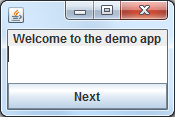
\includegraphics[width=0.9\linewidth]{images/swing-demo-step1.png} \\[1cm] 
Step2:\\
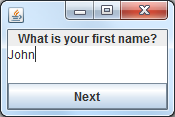
\includegraphics[width=0.9\linewidth]{images/swing-demo-step2.png} \\[1cm]
Step3:\\
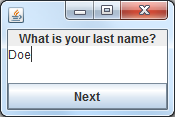
\includegraphics[width=0.9\linewidth]{images/swing-demo-step3.png} \\[1cm]
Step4:\\
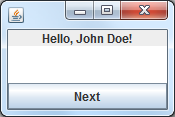
\includegraphics[width=0.9\linewidth]{images/swing-demo-step4.png} \\
\end{tabular}

    \end{minipage} 


\caption{A simple Scala-swing application with an asynchronous event-based control flow defined in a direct style.}
\label{fig:example_twelve_days}
\end{figure}










